\documentclass[crop,tikz]{standalone}

\usepackage[utf8]{inputenc}

% 'crop' is the default for v1.0, before it was 'preview'
%\usetikzlibrary{...}% tikz package already loaded by 'tikz' option

\newcommand{\eps}{\varepsilon}
	
\begin{document}

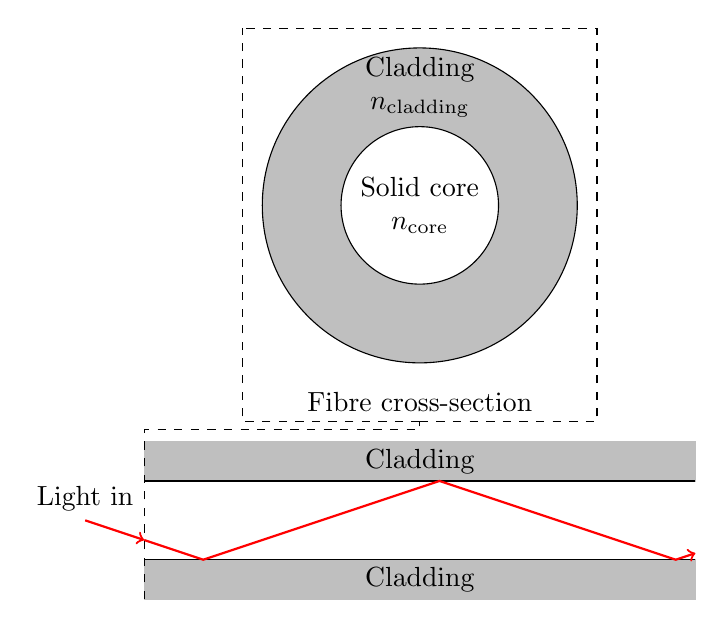
\begin{tikzpicture}
	%cross-section
	\begin{scope}[scale=1.0, shift={(0,0.5)}]
		\draw[fill=black!50!white!50!] (0,0) circle (2);
		\draw[fill=white] (0,0) circle (1);
		\node[anchor=center, align=center] at (0,1.5) {Cladding \\ $n_{\mathrm{cladding}}$};
		\node[anchor=center, align=center] at (0,0) {Solid core \\ $n_{\mathrm{core}}$};
	\end{scope}

	%guidance down fibre
	\begin{scope}[scale=1.0, shift={(-3.5,-3)}]
		\filldraw[black!50!white!50!] (0,0) rectangle (7,0.5);
		\draw (0,0) -- (7,0);
		\filldraw[black!50!white!50!] (0,-1) rectangle (7,-1.5);
		\draw (0,-1) -- (7,-1);
		%labels for cladding again
		\node[anchor=center] at (3.5,0.25) {Cladding};
		\node[anchor=center] at (3.5,-1.25) {Cladding};
		%light beam in
		\draw[thick, ->, red] (-0.75,-0.5) -- (0,-0.75);
		\node[anchor=south] at (-0.75,-0.5) {Light in};
		%beam via TIR
		\draw[thick, ->, red] (0,-0.75) -- (0.75,-1) -- (3.75,0) -- (6.75,-1) -- (7,-1+0.25/3);
	\end{scope}
	
	%connect cross-section with guidance diagram
	\begin{scope}[scale=1.0, shift={(-3.5,-3)}]
		\draw[dashed] (0,-1.5) -- (0,0.65) -- (3.5,0.65) -- (3.5,0.75);
		\draw[dashed] (3.5,0.75) -- (1.25,0.75) -- (1.25,5.75);
		\draw[dashed] (3.5,0.75) -- (5.75,0.75) -- (5.75,5.75) -- (1.25,5.75);
	\end{scope}
	
	\node[anchor=center] at (0,-2) {Fibre cross-section};
\end{tikzpicture}

\end{document}